% !TeX root = main.tex
\chapter{The Gemmini DNN Accelerator: An Architectural Overview}
\label{chap:gemmini_overview}

As established in the previous chapter, the System-on-Chip (SoC) developed in this thesis utilizes a single \texttt{Rocket} Core augmented with a specialized accelerator for deep learning workloads. This chapter delves into the high-level architecture of this accelerator: \texttt{Gemmini}. 

\begin{figure}[htbp]
    \centering
    
\includegraphics[width=0.9\textwidth]{Gemmini_Logo.pdf}
    \caption{Gemmini Logo. Source: \cite{gemini-dac}.}
    \label{fig:gemmini_logo}
\end{figure}

\section{Introduction to Gemmini}
\label{sec:gemmini_intro}

\texttt{Gemmini} is an open-source, full-stack Deep Neural Network (DNN) accelerator generator developed at the University of California, Berkeley \cite{gemini-dac}. It is designed not merely as a standalone hardware component, but as a complete ecosystem for exploring and evaluating domain-specific hardware acceleration. 

A key philosophy behind \texttt{Gemmini} is the concept of "full-stack" evaluation. Many DNN accelerators are designed and tested in isolation, which fails to account for critical system-level effects such as memory bus contention, cache coherency overhead, and operating system interactions (e.g., page faults and context switches) \cite{gemini-dac}. By generating not only the accelerator RTL but also a complete, Linux-capable SoC using the \texttt{Chipyard} framework, \texttt{Gemmini} enables a comprehensive evaluation of these cross-stack interactions. This allows for a more realistic assessment of performance and energy efficiency, making it a powerful tool for academic research. For this thesis, leveraging \texttt{Gemmini} provides the opportunity to explore a powerful DNN accelerator within a realistic SoC environment.

\section{Core Architectural Components}
\label{sec:gemmini_core_components}

The \texttt{Gemmini} generator can produce a wide range of accelerator instances based on a flexible architectural template. The core components, shown in Figure~\ref{fig:gemmini_template}, are detailed below.

\begin{figure}[htbp]
    \centering
    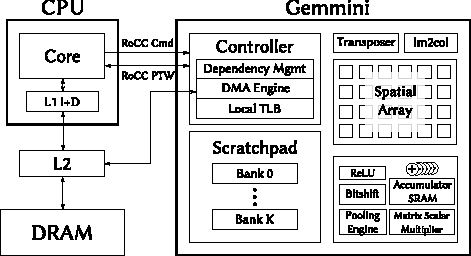
\includegraphics[width=0.9\textwidth]{Gemmini_ArchitectureOverview.pdf}
    \caption{High-level overview of the Gemmini accelerator template integrated with a host CPU and system memory hierarchy. Source: \cite{gemini-dac}.}
    \label{fig:gemmini_template}
\end{figure}

\subsection{The Systolic Array (Spatial Array)}
\label{subsec:systolic_array}

The computational heart of \texttt{Gemmini} is its systolic array, also referred to as a spatial array. This component consists of a 2D grid of Processing Elements (PEs), each capable of performing a Multiply-Accumulate (MAC) operation in a single cycle. The systolic array is highly configurable, with key parameters including:
\begin{itemize}
    \item \textbf{Dimensions:} The number of rows and columns in the PE grid (e.g., 16x16, 32x32) can be specified at generation time.
    \item \textbf{Dataflow:} \texttt{Gemmini} primarily supports two dataflow strategies: Weight Stationary (WS) and Output Stationary (OS). In WS dataflow, the DNN weights are pre-loaded into the PEs and remain stationary, while input activations are streamed through. This maximizes weight reuse. In OS dataflow, partial sums of the output activations remain stationary within the PEs, while inputs and weights are streamed. This is beneficial for layers with low weight reuse. The choice of dataflow has a significant impact on performance and energy efficiency.
    \item \textbf{Pipelining:} The degree of pipelining within the array and the PEs can be configured, affecting the maximum clock frequency and throughput.
\end{itemize}
This configurable systolic array allows \texttt{Gemmini} to efficiently execute the dense matrix multiplications that are fundamental to modern DNNs, especially for convolutional and fully-connected layers.

\subsection{On-Chip Memory Hierarchy}
\label{subsec:gemmini_onchip_mem}

To feed the high-throughput systolic array and avoid becoming memory-bound, \texttt{Gemmini} includes a dedicated on-chip memory hierarchy.
\begin{itemize}
    \item \textbf{Local Scratchpad Memory:} This is a software-managed SRAM used for staging input activations, weights, and intermediate feature maps close to the systolic array. Its purpose is to reduce the latency and energy consumption associated with fetching data from higher levels of the memory hierarchy, such as the shared L2 cache or main memory (DRAM). Its capacity and banking are configurable.
    \item \textbf{Accumulator Memory:} Separate from the main scratchpad, \texttt{Gemmini} features a dedicated memory to store the partial sums generated by the MAC operations. This memory typically uses a higher precision data type (e.g., 32-bit integers) than the input data (e.g., 8-bit integers) to maintain accuracy during accumulation.
\end{itemize}

\subsection{Integration as a RoCC Accelerator}
\label{subsec:gemmini_rocc}

As discussed in Chapter 3, \texttt{Gemmini} is designed to be integrated as a Rocket Custom Coprocessor (\texttt{RoCC}). This enables tight coupling with the host \texttt{Rocket} Core, allowing it to be controlled via custom RISC-V instructions dispatched by the core's main pipeline. 

This integration uses a decoupled access-execute model, as illustrated conceptually in Figure~\ref{fig:decoupled_pipelines}. The host CPU issues three main types of commands to \texttt{Gemmini}: load (from main memory to scratchpad), execute (perform computation on data within the scratchpad), and store (from scratchpad to main memory). These commands are placed into separate hardware queues, allowing \texttt{Gemmini}'s DMA engine to handle data movement in parallel with the systolic array's computations. This overlapping of communication and computation is crucial for hiding memory latency and maximizing the utilization of the systolic array.

\begin{figure}[htbp]
    \centering
    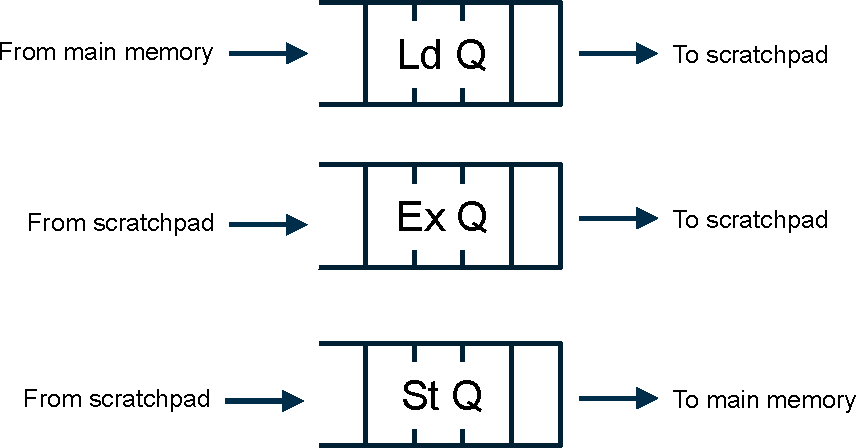
\includegraphics[width=0.8\textwidth]{Gemmini_DecoupledAccessExecutePipeline.pdf}
    \caption{Conceptual view of Gemmini's decoupled access-execute pipelines, managed by separate hardware command queues for Load, Execute, and Store operations. Source: \cite{gemini-dac}.}
    \label{fig:decoupled_pipelines}
\end{figure}

\section{Summary}
\label{sec:gemmini_overview_summary}
In summary, \texttt{Gemmini} is a sophisticated, highly configurable DNN accelerator generator. Its key architectural features include a powerful systolic array, a dedicated on-chip memory hierarchy, and a tightly-coupled integration with a host processor via the \texttt{RoCC} interface. This design enables the high-performance execution of DNN workloads within a full-stack, system-level context. 

Having established this high-level architectural overview, the following chapter will now perform a deep dive into the specifics of \texttt{Gemmini}'s internal command processing flow and its multi-level programming model.